\documentclass[11pt]{article}
\usepackage{graphicx} % To include graphics 
\usepackage[tbtags]{amsmath} % tbtags to make eq number at last line
\usepackage{amssymb}
%\usepackage{wrapfig} % For figures next to text
\usepackage{booktabs} % Better tables
% \usepackage{physics} 
\usepackage{cases} % For cases with separate labels
\usepackage{hyperref}% For cross-referencing
\hypersetup{colorlinks=true, linkcolor=blue, urlcolor=blue, citecolor=blue}
%\usepackage{pgfplots} % For drawing graphs
\usepackage{parskip} % To remove indentation and set paragraph spacing
\usepackage[margin=1in]{geometry}
%\usepackage{cancel} % To cancel out terms
\usepackage{listings} % To write code
\usepackage{xcolor} % To write color text/math by \textcolor{color}{text}
\usepackage{enumitem} % Better list environment
\usepackage{fancyhdr} % For custom headers and footers
% \usepackage{amsthm} % To write theorems and proofs
% \renewcommand\qedsymbol{$\blacksquare$}
% \usepackage{algorithm}
% \usepackage{algpseudocode}

%%%%%%%%%% Configure fancy headers %%%%%%%%%%
\pagestyle{fancy}

%%%%%%%%%% listings config (for writing code) %%%%%%%%%%
% \definecolor{codegreen}{rgb}{0,0.6,0}
% \definecolor{codegray}{rgb}{0.5,0.5,0.5}
% \definecolor{codepurple}{rgb}{0.58,0,0.82}
% \definecolor{backcolour}{rgb}{0.95,0.95,0.92}

% \lstdefinestyle{mystyle}{
%     frame=tb,
%     basicstyle=\ttfamily,
%     backgroundcolor=\color{backcolour},   
%     % commentstyle=\color{codegreen},
%     % keywordstyle=\color{magenta},
%     % stringstyle=\color{codepurple},
%     breakatwhitespace=false,         
%     breaklines=true,                 
%     captionpos=b,                    
%     keepspaces=true,                 
%     numbers=left,                    
%     numbersep=5pt,                  
%     showspaces=false,                
%     showstringspaces=false,
%     showtabs=false,                  
%     tabsize=4
% }
% \lstset{style=mystyle}

% Title
\title{CSCI3100 Project Design And Implementation}
\author{
    \textbf{Group 17} \\[1em]
    \begin{tabular}{ll}
        Ng Ching Yin & (1155175606) \\
        Lam Hoi Chun & (1155192755) \\
        Lai Wing Fai & () \\
        Zou Zhihong & (1155204947)
    \end{tabular}
}
\date{\today}

\begin{document}
\maketitle

% Table of contents
{
    \hypersetup{linkcolor=black}
    \tableofcontents
}

\newpage

% Document Revision History
% Update this only before pull request, don't update every commit
\section{Document Revision History}
\begin{table}[h]
    \centering
    \caption{Document Revision History}
    \begin{tabular}{cccc}
        \toprule
        Version & Revised By & Revision Date & Comments \\
        \midrule
        0.0.1 & Ng Ching Yin & 31 Oct 2025 & Initial draft \\
        \bottomrule
    \end{tabular}
    \label{tab:docs_rev_hist}
\end{table}

% Introduction
\section{Introduction}

\subsection{Purpose}

This document describes the architecture, system and user interface design for devban, a
software project management tool. This document will serve as a basis for developers
to implement the features in the application.

\subsection{Scope}

This document describes the design and implementation details of the devban
Application. This document will focus on four components: 
database, user management, UI design and implementation of the main features. 
Each of the components will be explained in details.

\subsection{Definitions, Acronyms and Abbreviations}
\begin{table}[h]
    \centering
    \caption{Definitions, Acronyms and Abbreviations}
    \begin{tabular}{p{2cm} p{12cm}}
        \toprule
        Acronyms
        & Description \\
        
        \midrule
        devban
        & Name of the project, shortened from ``developers'' and ``kanban'' \\

        \midrule
        UI
        & User Interface \\

        \midrule
        GUI
        & Graphical User Interface \\

        \midrule
        MVVM
        & Model-View-ViewModel \\

        \midrule
        idP
        & Identity provider \\
 
        \bottomrule
    \end{tabular}
    \label{tab:docs_definitions_acronyms_and_abbreviations}
\end{table}


\section{System Overview}

devban offers multiple useful features, including kanban board for resource management and
progress tracking, calendar for visual planning, messaging for communication and LLM interface
to boost development productivity. On top of that, it provides a graphical user interface that 
enables users to interact with the system easily. Furthermore, gamification elements are to serve
as a motivation-boost for users.

\section{System Architecture}

\subsection{Architecture Design}

The application will follow the Model-View-ViewModel (MVVM) design pattern, where
View represents the graphical user interface (GUI), Model controls the business logic, and
ViewModel acts as a middleman to controls the view updates and send API request to the model.

\subsection{Decomposition Description}
Figure \ref{fig:decomposition_description} shows a high level decomposition of the components in devban. 
Users interact with the system via a GUI, which forward the actions to the view models and models.
The view models will then update the views according to the action and the data from database.

Some external services are used to extend the system capabilities:
\begin{itemize}%[leftmargin=*]
    \item external identity provider (idP) are used to provide secure user authentication;
    \item LLM Provider API are used to get access to advanced LLM models;
\end{itemize}

\begin{figure}[h]
    \centering
    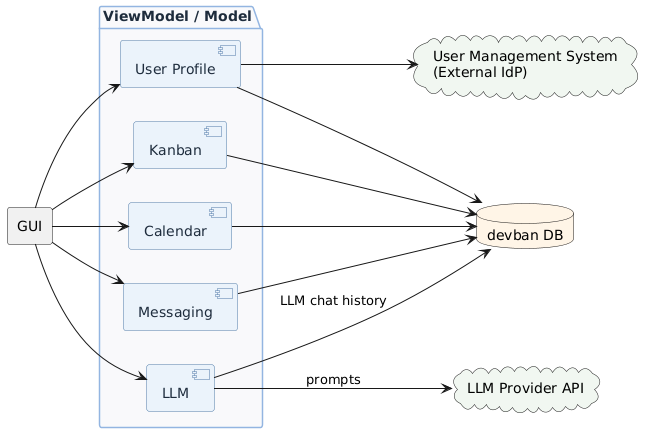
\includegraphics[width=0.8\textwidth]{assets/system_architecture/system_architecture.png}
    \caption{Components diagram for high level overview of devban application.}
    \label{fig:decomposition_description}
\end{figure}


% \appendix
% \addcontentsline{toc}{section}{Appendix}
% \section*{Appendix}
% \section{References}

\end{document}